\chapter{Directed caused accompanied motion} \label{ch:CAM}

%is cam.verb-DIR much more common that I recorded? go through all 70 languages to check data? 

%Dryer 136
%It is not always clear, however, whether a morpheme is adding a separate motion
%event. One situation where there can be uncertainty is cases where a verb is glossed
%with something like `carry, take, bring'. Consider (16) from Huasteca Nahuatl.
%In (16), a ventive suffix (glossed `come') combines with a verb glossed as `bring'.
%One possibility is that the ventive suffix here is simply a directional, coding the
%direction of the bringing. The English verb bring is inherently ventive, but there
%are other Huasteca Nahuatl examples cited by Beller and Beller (1979) with the
%same verb walika that occurs in (16) but which Beller and Beller gloss as `take', so
%it could be that it is really the ventive suffix that yields the meaning `bring' rather
%than `take'.
%If the verb walika really does represent a motion event, then the ventive suffix
%in (16) is probably best viewed as a directional. However, a second possibility
%is that the event of bringing and the event of coming should be considered two
%separate motion events, in which case the ventive suffix in (16) is a marker of AM,
%not a directional. We must be careful, however, not to read too much into the
%way a verb is glossed. The English verbs carry, take, and bring all inherently code
%motion, but there may be cases where a verb that is glossed as `carry', `take' or
%`bring' can be used to include instances of holding, where there is no motion. If a
%ventive or andative morpheme combines with a verb of this sort, then it probably
%should be treated as a marker of AM rather than as a directional. In this chapter,
%I treat morphemes that combine with verbs glossed as `carry' or `take' as directionals rather than as markers of AM. However, some of these cases may turn
%out to be cases where the verb can mean something like `hold', in which case the
%morpheme should be treated as a marker of AM.

This chapter examines one functional domain in which some Chadic languages use directional extensions, namely, the expression of directed caused accompanied motion (e.g., `bring (here)', `take away'). By examining what means are used cross-linguistically to express a particular function, the use of directional extensions in this context is put into perspective as one morphosyntactic strategy among several that are found in various Chadic languages. 

\section{Expressing directed caused accompanied motion}

\citet{hellwigBringingTakingCrosslinguistic2022} introduce the notion of caused accompanied motion (CAM) as a cover term for the study of linguistic descriptions of bringing and taking events.  They focus on CAM events that are described as happening in a particular direction: directed CAM. They analyze directed CAM events as including four components of meaning: (translocative) motion, causation, accompaniment and directedness. Directed CAM events are frequently expressed through specialized morphosyntactic means. Among the morphosyntactic means for expressing directed CAM, \citet{hellwigBringingTakingCrosslinguistic2022} include four that are commonly found in Chadic languages. 

First, all components of directed CAM (including the directional component) may be expressed in a single verb root, as in the Barayin ventive CAM verb root \textit{sar} `bring' in (\ref{ex:bara0}), which contrasts with the Barayin itive CAM verb root \textit{kor} `take away'. This means for expressing directed CAM is discussed in \sectref{sec:dcamverb}.

\ea\label{ex:bara0}
\langinfo{\hyperref[bara]{Barayin} directed (ventive) CAM verb \textit{sar-} `bring' }{}{\cite[128]{lovestrandLinguisticStructureBarain2012}} \\
\gll kà sár-gì dō \\
3\gl{sg}.\gl{m}.\gl{sbj} bring-3\gl{sg}.\gl{m}.\gl{obj} \gl{neg} \\
\glt `He didn't bring it.'
\z

Second, a verb root which expresses general (non-directional) caused accompanied motion (e.g., `carry') may be modified by an additional element to express direction, as in the use of ventive directional morphology in (\ref{ex:kare8}). The use of this means for expressing directed CAM is discussed in \sectref{sec:modcamverb}.

\ea\label{ex:kare8}
\langinfo{\hyperref[kare]{Karekare} verb \textit{wula} `carry' with ventive suffix}{}{\cite[]{abareTCNN16Suleiman2016}} \\
\gll mendau yi 'wule-ne waɗa a mizitau \\
woman the carry-\gl{vent} food \gl{prep} male	\\
\glt `The woman brought food to her husband.'
\z 

Third, a directional motion verb may be modified to include the causation and accompaniment components of directed CAM meaning. This modification can be syntactic, as in the use of a comitative prepositional phrase in \hyperref[peve]{Pévé}, shown in (\ref{ex:peve7}), or it can be morphological, as in the use of a causative suffix in \hyperref[lama]{Lamang}, shown in (\ref{ex:lama09}). These means for expressing directed CAM are discussed in \sectref{sec:dirCAM}.

\ea\label{ex:peve7}
\langinfo{\hyperref[peve]{Pévé} directional verb with prepositional phrase}{}{\cite[217]{shayGrammarPeve2020}} \\
\gll ha mbə́ kə sə̀lày si su \\
2.\gl{m} come \gl{asoc} money \textsc{assertive} \gl{q} \\
\glt `Did you bring (lit. `come with') money?'

\ex\label{ex:lama09}
\langinfo{\hyperref[lama]{Lamang} directional verb with causative suffix}{}{\cite[142]{wolffLamangLanguageDictionary2015}} \\
\gll sá-ŋá-ghà \\
come-\gl{caus}-\gl{home} \\
\glt `bringing home'
\z 

Fourth, the use of a verb of acquisition (e.g., `take', `get') may be modified by a directional extension in order to express directed CAM, as in the ventive form of the verb \textit{hàw} ‘take' in \hyperref[kera]{Kera}, shown in (\ref{ex:kera06}). The use of this means for expressing directed CAM is discussed in \sectref{sec:takecam}.

\ea\label{ex:kera06}
\langinfo{\hyperref[kera]{Kera} verb \textit{hàw} ‘take' with ventive suffix}{}{\cite[116]{ebertSpracheUndTradition1979}} \\
\gll hàw-dà 	\\
take-\textsc{vent}	\\
\glt `Bring it here!'
\z 

\largerpage
To summarize, the four morphosyntactic means for expressing directed CAM that are examined for Chadic languages in this chapter are as follows:

\begin{enumerate} \itemsep0em 
	\item	Directed CAM verb root (e.g., `bring')
	\item	CAM verb root (e.g., `carry') + directional extension 
	\item	Directional verb root (e.g., `go', `come') + valency-increasing morphosyntax 
	\item	Verb of acquisition (e.g., `get', `take') + directional extension
\end{enumerate}

\tabref{tab:CAM} shows the number of languages (by branch) in which each of the four strategies for expressing directed CAM appear. For this study, a subset of 79 languages were included as the remaining languages were not considered to have sufficient information available to make any judgment on how directed CAM is expressed in the grammar. In 21 languages, more than one morphosyntactic means of expressing CAM are attested, so the totals  in \tabref{tab:CAM} show 100 means of expressing CAM across 79 languages. For nine of the 79 languages, no evidence of a morphosyntactic means of expressing directed CAM was found in the available data. The geographic distribution of these strategies for expressing directed CAM in Chadic languages is shown in \figref{fig:CAM}.

%data in tab:verbsbranch is from python code in file CAM 
\begin{table}
	\caption{Forms of directed CAM in Chadic languages (by branch)}
	\label{tab:CAM}
	\begin{tabularx}{\textwidth}{l Yrrr Y}
		\lsptoprule
{} &  West (21) &  Biu-M. (41) &  Masa (3) &  East (13) & Total \\
\midrule
Directed CAM verb     &     0 &            6 &     0 &     2 & 8 \\
Modified CAM verb &     4 &            9 &     0 &     0 & 13\\
Modified DIR verb   &    14 &           16 &     2 &     5 & 37 \\
Modified TAKE verb   &     6 &           25 &     1 &     1 & 32 \\
Not found     &     2 &            2 &     0 &     5 & 9 \\
\midrule
Total    &    26 &           58 &     3 &    13 & 100 \\
		\lspbottomrule
	\end{tabularx}
\end{table}

%see R code in file 'CAM map R code' 
\begin{sidewaysfigure}
	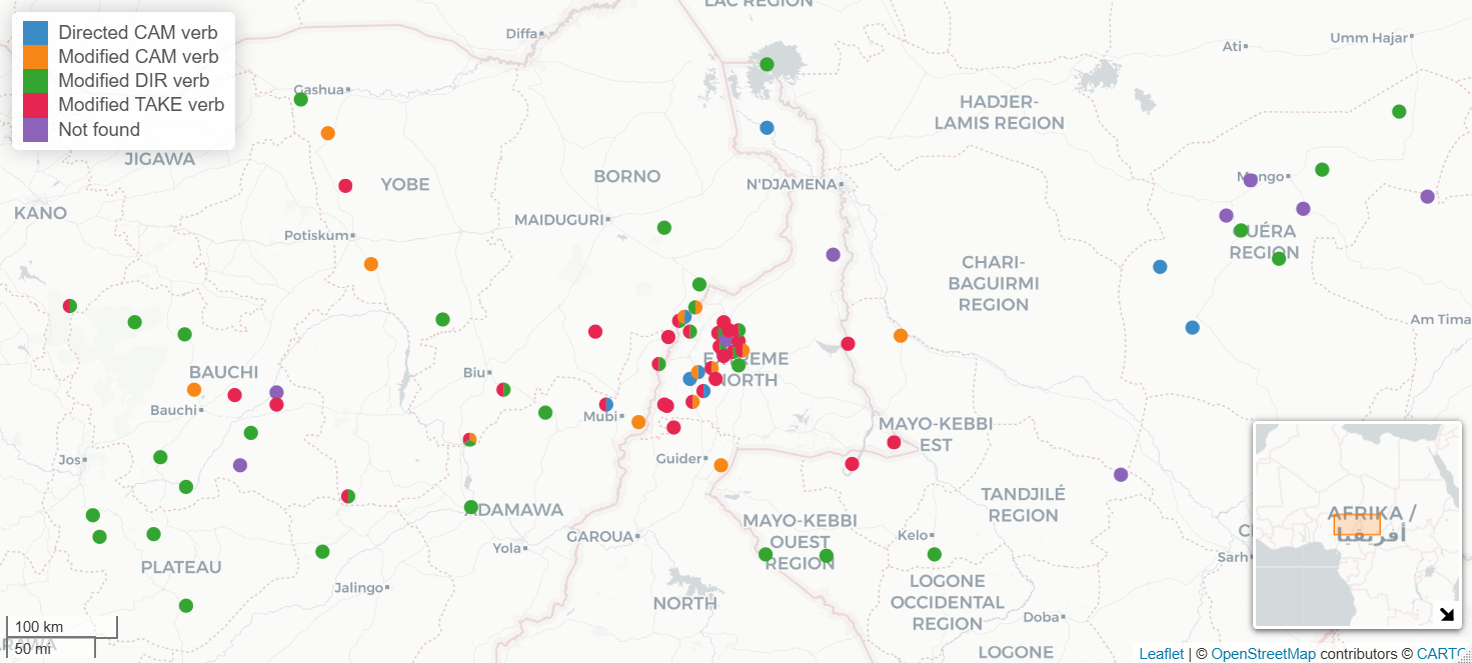
\includegraphics[width=\textwidth]{maps/CAM.png}
	\caption{Geographic distribution of forms for expressing directed CAM} \label{fig:CAM}
\end{sidewaysfigure}

\citet{hellwigBringingTakingCrosslinguistic2022} also discuss multiverb constructions used for the expression of directed CAM \citep[see also][104--106]{lovestrandSerialVerbConstructions2021a}. Multiverb constructions are not included in this study of Chadic languages due to the limited number of available descriptions. However, in those cases where grammatical descriptions do include multiverb constructions, no directed CAM functions are discussed.\footnote{Descriptions of multiverb constructions in Chadic languages include \citet[185--189]{shayGrammarPeve2020} on \hyperref[peve]{Pevé}, \citet[445]{frajzyngierGrammarGidar2008} on \hyperref[gida]{Gidar}, \citet[409]{allisonGrammarMakaryKotoko2020} on \hyperref[maka]{Makary Kotoko}, \citet[146]{wolffLamangLanguageDictionary2015} on \hyperref[lama]{Lamang}, \citet[210]{hoffmannGrammarMargiLanguage1963} on \hyperref[marg]{Margi}, \citet[269]{friesenGrammarMoloko2017} on \hyperref[molo]{Moloko}, \citet[215--218]{shayGrammarGizigaChadic2021} on \hyperref[gizi]{Giziga}, \citet[65]{viljoenGavarVerbPhrase2017} on \hyperref[gava]{Gavar}, \citet[2--3]{lienhardDabaGrammarClause1978} on \hyperref[daba]{Daba}, \citet[373--376]{frajzyngierGrammarMina2005} on \hyperref[mina]{Mina}, \citet[131--134]{thomasGrammarSakunSukur2014} on \hyperref[saku]{Sakun}, \citet[183--187]{frajzyngierGrammarLele2001} on \hyperref[lele]{Lele}, \citet[217]{peustSupplementsWestDangla2016} on \hyperref[dang]{Dangla}, \citet[250]{frajzyngierGrammarPero1989} on \hyperref[pero]{Pero}, \citet[412]{hellwigGrammarGoemai2011} on \hyperref[goem]{Goemai}, and \citet{lovestrandSerialVerbConstructions2018} on \hyperref[bara]{Barayin}. The most commonly reported function of multiverb constructions is the expression of prior motion, as is also commonly found cross-linguistically \citep{lovestrandSerialVerbConstructions2021a}.} This suggests that multiverb constructions are not a common syntactic structure used for expressing directed CAM in Chadic languages.

\section{Verb root expressing directed CAM} \label{sec:dcamverb}

The use of a directed CAM verb root is the least frequently attested means of expressing directed CAM, found in only eight languages.\footnote{These numbers potentially reflect under-reporting in the available data. Verb roots were only counted as lexicalization of directed CAM where the evidence made it clear that the verb stem could not be used as a general (non-directional) CAM verb (e.g., `carry') or as a verb of possession (e.g., `take'). General CAM verbs and verbs of possession are discussed separately as they often take on directed CAM meanings when modified by a directional extension.} In four of those languages, both a ventive and an itive CAM verb root are attested. In the other four languages, the only attested directed CAM verb root is ventive. The forms of directed CAM verb roots in the data are shown in \tabref{tab:dcamverbs}.

\begin{table}
	\caption{Forms of directed CAM verb roots} 
	\label{tab:dcamverbs}
	\begin{tabular}{llll} % add l for every additional column or remove as necessary
		\lsptoprule
		Language & Branch & VENT CAM & ITIVE CAM   \\ %table header
		\midrule
		\hyperref[dghw]{Dghwede} & Biu-Mandara & \textit{náxa} & \\
		\hyperref[maka]{Makary Kotoko} & Biu-Mandara & \textit{ɗō} &  \textit{do}  \\
		\hyperref[buwa]{Buwal} & Biu-Mandara & \textit{dā} & \textit{ɮāɗ} \\
		\hyperref[gava]{Gavar} & Biu-Mandara & \textit{daa} & \textit{dʒaɓ} \\
		\hyperref[mbud]{Mbudum} & Biu-Mandara & \textit{daha} & \\
		\hyperref[huba]{Huba} & Biu-Mandara & \textit{shìlnì} & \\
		\hyperref[bara]{Barayin} & East &  \textit{sèeró}, \textit{ajuro} & \textit{kóoro} \\
		\hyperref[soko]{Sokoro} & East & \textit{aaya} &  \\
		\lspbottomrule
	\end{tabular}
\end{table}

Three closely related Biu-Mandara languages, \hyperref[buwa]{Buwal}, \hyperref[gava]{Gavar} and \hyperref[mbud]{Mbudum}, show similar forms of verb roots for expressing directed CAM. There is likely an etymological link between the forms of these ventive CAM verbs and the ventive extension \textit{aha} which is still productive in these three languages. In \hyperref[bara]{Barayin}, there is a transparent etymological relationship between the directed CAM verb roots and the directional verb roots \textit{kóló} `go', \textit{ājó} `come' and \textit{síi} `come'. The stem-final \textit{-r} is probably from an erstwhile ``oblique'' suffix which likely had a valency increasing function \citep{robertsObliquesMawa2016}. 

In four of the seven languages with directed CAM verb roots, this strategy exists alongside another morphosyntactic means of expressing directed CAM. In \hyperref[buwa]{Buwal} and \hyperref[dghw]{Dghwede}, there is also evidence that general CAM verb roots can be modified by a directional extension to express directed CAM (\sectref{sec:modcamverb}). In \hyperref[mbud]{Mbudum} and \hyperref[huba]{Huba}, it is also possible to express directed CAM using a modified `take' verb (\sectref{sec:takecam}).

\section{Modified CAM verb} \label{sec:modcamverb}

In at least 13 languages, directed CAM may be expressed by a general CAM verb root (e.g., `carry', `transport') modified by a directional extension. For example, in \hyperref[bole]{Bole}, the general CAM verb root \textit{àlā} `carry, take from one place to another' has a ventive form \textit{èlen} `bring' \citep{gimbaBoleenglishhausaDictionaryAlhaji2004}. This may be an under-reported strategy, as many descriptions of languages with directional extensions only provide a limited number of examples. The absence of examples of CAM verbs modified by a directional extension may be a gap in the data. In regard to East Chadic languages, there are very few languages with directional extensions, so it is unsurprising that this strategy for expressing directed CAM is not reported in the East Chadic branch. 

In six languages, the use of a modified CAM verb appears to be the only morphosyntactic means of expressing directed CAM (in the available data). In the other seven languages, at least one of the other three strategies for expressing directed CAM are also attested. 

\section{Modified directional verb} \label{sec:dirCAM}

Nearly half of the languages in the sample, 37 of 79, can use a modified directional verb root (e.g., `come', `go') to express directed CAM. These can be divided into two categories. In 13 languages, the transported item is expressed in a prepositional phrase, as in (\ref{ex:nyam2}) and (\ref{ex:lele16}). In many languages, this preposition is identified as an associative preposition, as in (\ref{ex:lele16}). Associative is a label used in Chadic languages for a comitative preposition that also conjoins noun phrases. 

\ea\label{ex:nyam2}
\langinfo{\hyperref[nyam]{Nyam} verb \textit{tò} `come' with comitative prepositional phrase}{}{\cite[127]{andreasGrammatischeBeschreibungNyam2012}} \\
\gll mùdùk tò-wá yà kɔ̀lɔ́ŋ \\
woman come-\textsc{perf} with food \\
\glt `The woman has brought food.'

\ex\label{ex:lele16}
\langinfo{\hyperref[lele]{Lele} verb \textit{èje} `come' with associative prepositional phrase}{}{\cite[203]{frajzyngierGrammarLele2001}} \\
\gll èje dí ná kama \\
come 3\gl{sg} \gl{asoc} water \\
\glt `He brought water.'
\z 

In the other 24 languages, the directional verb root is used transitively so that the object of the verb is the transported item in the directed CAM event. Where directed CAM is expressed through increasing the valency of a directional motion verb, this is often described as a function of causative morphology, as in (\ref{ex:budu3}) and (\ref{ex:lama9}). In (\ref{ex:lama9}) the verb is further modified by an upward directional. 

\ea\label{ex:budu3}
\langinfo{\hyperref[budu]{Buduma} verb \textit{wú} `come' with causative suffx}{}{\cite[61]{lukasSpracheBudumaIm1939}} \\
\gll u-wú-re̤ \\
1\gl{sg}-come-\gl{caus} \\
\glt `I bring.' [German: `\textit{Ich bringe.}']

\ex\label{ex:lama9}
\langinfo{\hyperref[lama]{Lamang} verb \textit{s} ‘come’ with causative suffixes}{}{\cite[142]{wolffLamangLanguageDictionary2015}} \\
\gll
sá-ŋé-fé \\
come-\gl{caus}-\gl{up} \\
\glt `bringing up'
\z 

In other cases, verbal morphology with a similar function is described as marking transitivity rather than causation, as in the case of \hyperref[malg]{Malgwa} in (\ref{ex:malg13}). Alternatively, a valency-increasing suffix with a similar function may be described as an ``oblique'' marker \citep{robertsObliquesMawa2016}. Further comparative study would be needed to determine if there is any substantial variation in the functions of verbal morphology labeled `causative', `transitive' or `oblique'. 

\ea\label{ex:malg13}
\langinfo{\hyperref[malg]{Malgwa} verb \textit{d} `go' with transitive and outward suffixes}{}{\cite[139]{lohrSpracheMalgwaNara2002}} \\
\gll d-an-sé \\
go-\gl{tr}-\gl{out} \\
\glt `take away' [German: `\textit{wegnehmen}']
\z 

In at least two languages, \hyperref[mafa]{Mafa} and \hyperref[mbuk]{Mbuko}, directional verbs are labile and can be used in transitive contexts (expressing directed CAM) with no valency-increasing morphology on the verb, as in (\ref{ex:mbuk5}) where the noun phrase headed by \textit{zana} `cloth' is the direct object of the directional verb \textit{zla} `go'. 

\ea\label{ex:mbuk5}
\langinfo{\hyperref[mbuk]{Mbuko} verb \textit{zla} `go' as a transitive predicate}{}{\cite[22]{gravinaVerbPhraseMbuko2001}} \\
\gll Ta-zla anan zana a-tinen ahay pə-tila aga njavan ahay\\
3\gl{pl}.\gl{pfv}-go \gl{foc} cloth of-they \gl{pl} on-tailor house.of guinea-fowl \gl{pl}\\
\glt `They took their clothes from the tailor to the guinea-fowls’ house.'
\z 

\section{TAKE verb with a directional extension} \label{sec:takecam}

Besides modifying a directional verb, the other common strategy for expressing directed CAM is through the combination of a verb of possession (often glossed as `take') combined with a directional extension, as in (\ref{ex:haus7}) and (\ref{ex:mata12}).

\ea\label{ex:haus7}
\langinfo{\hyperref[haus]{Hausa} verb \textit{kāw} `take' with ventive extension}{}{\cite[663]{newmanHausaLanguageEncyclopedic2000}} \\
\gll kāw-ō \\
take-\gl{vent} \\
\glt `bring'

\ex\label{ex:mata12}
\langinfo{\hyperref[mata]{Matal} verb \textit{xə̀l} `take' with ventive extension}{}{\cite[294]{dougopheGrammarMatal2021}} \\
\gll  tá-xə̀l gwàʦàk àwáŋ áŋà  mà-ʦə̀ɗ-àj 	\\
3.\gl{pl}-take hen \gl{vent} \gl{purp} \gl{inf}-cut-??		\\
\glt `They bring a hen to slaughter...'
\z 

In languages with multiple directional extensions, it is possible for directionals other than ventive to be used to specify the direction of a CAM event, as in the use of the \hyperref[lama]{Lamang} downward suffix in (\ref{ex:lama12}). 

\ea\label{ex:lama12}
\langinfo{\hyperref[lama]{Lamang} verb \textit{ksa} ‘catch’ with downward extension}{}{\cite[78, 153]{wolffLamangLanguageDictionary2015}} \\
\gll ksa-gáa-tá	\\
catch-\gl{down}-\gl{compl}		\\
\glt `catching and taking downhill'
\z 

The strategy of modifying a `take' verb is particularly common among Biu-Mandara languages (25/41, 61\%). The higher frequency of the use of `take' verbs to express directed CAM in Biu-Mandara languages corresponds to the frequency at which directional extensions are found in each branch. However, this does not mean that all languages with directional extensions use a modified `take' verb for expressing directed CAM. Of the 79 languages in this sample, 54 have directional extensions. The modified `take' verb strategy is attested in 33 (61\%) of those languages.

\section{Conclusion}

Given the range of possible ways of expressing directed CAM, even among related languages, it is worth exploring the factors that may explain the distribution of various strategies for expressing directed CAM in Chadic languages. Two strategies are most commonly found: the use of a modified `take' verb root and the use of a modified directional verb root. The other two strategies are more rarely found: a directed CAM verb root and a modified CAM verb root. 

There is a pattern that correlates with the use of `take' verb roots in this context. As discussed in Chapter \ref{ch:functions}, directional extensions are typically multifunctional and one of the most common functions alongside direction is the expression of subsequent associated motion\index{associated motion}. Depending on the semantics of the event, it is possible for the subsequent motion to include a caused accompanied motion meaning, as in (\ref{ex:mafa3}).

\ea\label{ex:mafa3}
\langinfo{\hyperref[mafa]{Mafa} verb \textit{ta} `cook' with ventive suffix}{}{\cite[46]{barreteauLexiqueMafaLangue1990}} \\
\gll  n ta-ká mávə́r tə gáy	\\
3\gl{sg}.\gl{acc} cook-\gl{vent} boule in hut \\
\glt `She cooked the boule in the hut and brought it.' \newline
[French: `\textit{Elle a cuit la boule de mil dans la case et l'a apportée}.']
\z

%number in this paragraph from phyton code in CAM file
There are 34 languages with a directional extension that co-expresses subsequent associated motion\index{associated motion}. These include 32 of 33 languages which use the modified `take' verb strategy to express directed CAM.\footnote{The one exception is \hyperref[gizi]{Giziga} where most examples with non-motion verbs do not provide any indications of the function of the ventive directional suffix.} Since the use of `take' verbs for directed CAM is correlated with the subset of languages in which directional extensions co-express subsequent motion, it can reasonably be stated that (for Chadic languages) the use of `take' verbs to express directed CAM is a natural extension of the subsequent motion interpretation of directional extensions. This explains why not all Chadic languages with directional extensions use this strategy. Not all Chadic languages co-express subsequent motion meaning with a directional extension. 

This pattern indicates that (in Chadic languages) the motion component of the CAM expression is derived from the directional extension, not from the `take' verb root. By this account, there is no need to assume that the verb roots involved in these constructions have any inherent translocative motion meaning \citep[see discussion in][]{narasimhanPuttingTakingEvents2012}. If verb roots glossed `take' are assumed to be motion verbs, then it would be difficult to explain why many Chadic languages that have a directional extension do not use a modified `take' verb to express directed CAM. The explanation is that these Chadic languages have not developed the co-expression of subsequent motion that allows the use of `take' verbs to express directed CAM.

The use of valency-increasing morphosyntax with directional motion verbs is the other common strategy for expressing directed CAM, but its distribution is more difficult to account for. According to  \citet[][9]{jaggarHausaGrade52014}, the existence of causative forms of directional verbs expressing directed CAM can be taken as evidence that CAM expressions are semantically the causative counterpart of intransitive motion.\footnote{Contrast this view with \citet[31]{dixonTypologyCausativesForm2000} who assumes that a form in Yidiny which elsewhere has a causative function should be considered an applicative when used with a motion verb to express CAM.} From this point of view, there is nothing surprising about the presence of this strategy for expressing directed CAM. However, if this where a (universal) semantic structure, then it would be difficult to explain why it is not used in many languages where it is morphosyntactically possible. In addition, \citet[14]{hellwigBringingTakingCrosslinguistic2022} point out that, in the expression of CAM, other means of increasing the valency of intransitive motion verbs are just as common (or more common) than causativization. The use of causative forms in the expression of CAM is just one of several ways in which valency-increasing strategies may be repurposed to express a salient function. These appear to be idiomatic combinations that extend the meanings of productive morphology, and should not necessarily be subjected to synchronic semantic decomposition.  

We can also ask why the other two directed CAM strategies are relatively rare. Given the prevalence of directional morphology in Chadic languages, it might be expected that the combination of directional extensions with general CAM verb roots (e.g., `carry') would be a more commonly attested strategy for expressing directed CAM. As mentioned above, the apparent infrequency of this strategy may be an accidental gap in the data. However, another possible explanation is that some general CAM verb roots also specify the manner in which an item is transported. This additional semantic detail may fit the description of some types of directed CAM events, but it could make this strategy less ideal for the more general function of describing directed CAM without regard to manner. 

In regard to the rarity of verb roots that express all of the semantic components of directed CAM events (e.g., `bring'), there may be a more widespread cross-linguistic dispreference for maintaining directed CAM verb roots in the lexicon. In their sample of 13 languages from diverse language families, \citet[11]{hellwigBringingTakingCrosslinguistic2022} identify only two languages that express directed CAM as a verb stem. 
